\chapter{Implementation}

PaWS is a very light and portable framework. This is achieved by using
multiple flexible and easy-to-extend technologies and tools, that are
presented in this section. All aspects related to the implementation
of PaWS are introduced with an architecture description and an
overview of specific solutions used. The last part of this chapter
contains information about problems encountered during the development
process.

This chapter must be read to understand how PaWS is working. It is
also a great introduction to Chapter 3, namely the configuration of
the PaWS framework.

\section{PaWS Architecture}

This section presents the general software architecture. At first, the
base and a high-level description of the architecture concept are
introduced. The next subsection describes elements of the PaWS framework
and their relationship. Scenarios of PaWS operations are also included.

\subsection{The \emph{Model-View-Controller} Design Pattern}
\label{mvc}

\begin{figure}[h!]
  \centering
  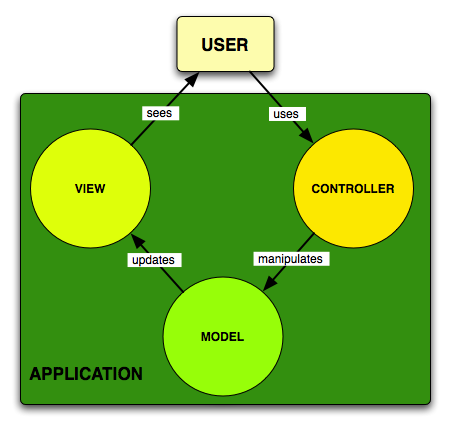
\includegraphics[width=0.5\textwidth]{reportCh2/mvc}
  \caption{MVC concept\cite{mvc_for_php}}
  \label{fig:mvc}
\end{figure}

PaWS is based on the MVC\cite{mvc} design pattern. MVC stands for
\emph{Model-View-Controller} and is an architectural design pattern
for software engineering, especially for creating applications with
graphical user interface.

As can be seen on Figure~\ref{fig:mvc}, MVC divides the application
into three parts:
\begin{itemize}

\item {\bf Model}, which is the representation of the problem or
  application logic,

\item {\bf View}, which describes how to display some parts of the model
  in the user interface,

\item and {\bf Controller}, which is responsible for communicating
  with the user, to update the model and refresh the view.

\end{itemize}

In PaWS framework, the Model layer is not present, because there is no
specific data logic and no database is used. However, PaWS could be
extended by adding, for example, a user authentication or a customization
for users (e.g. memorizing preferences) and, in this case, a database
(and a Model layer) will be necessary.

\subsection{Architecture Overview}

PaWS is a framework which provides its functions remotely. 
\begin{figure}[h!]
  \centering
  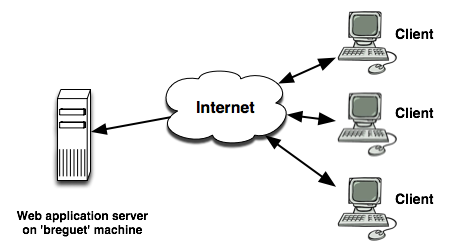
\includegraphics[width=0.5\textwidth]{reportCh2/web_applications}
  \caption{Architecture of access to web applications}
  \label{fig:web_applications}
\end{figure}
This means there is no need to install it on the client machine.  PaWS
can be reached via the Internet as it is shown in the Figure
\ref{fig:web_applications}. Clients need only a web browser - so
called \emph{thin client}. A \emph{Thin client} can be a terminal or a
computer. It needs another machine (its server) to perform its
tasks. Advantages of this approach are 1) no need to install special
tools on client machines, 2) independence from software changes on the
server and 3) low load of the clients machine.

Disadvantages of this solution may be: 1) a reduced functionality
on the client side, 2) the necessity of  an internet connection to
perform the tasks and 3) all of the usual limitations of a network,
latency and bandwidth.

In addition, undre PaWS, PIPS is running, as it is shown in
Figure~\ref{fig:webapp_paws}. What is more, Pyrops, which is described
in section \ref{other_technologies}, enables a remote usage of PIPS and
distribution of the application to balance the load.


\begin{figure}[h!]
  \centering
  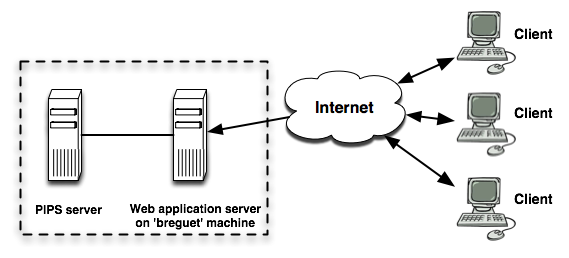
\includegraphics[width=0.5\textwidth]{reportCh2/webapp_paws}
  \caption{Architecture of access to PaWS}
  \label{fig:webapp_paws}
\end{figure}

PaWS architecture is not complicated. It consists of 3 layers,
presented in Figure \ref{fig:paws_architecture}.

\begin{figure}[h!]
  \centering
  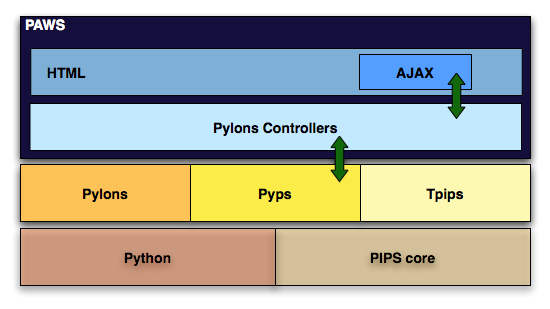
\includegraphics[width=0.7\textwidth]{reportCh2/paws}
  \caption{Architecture of PaWS}
  \label{fig:paws_architecture}
\end{figure}

The top layer is {\bf PaWS web application}. This blue layer consists in:

\begin{itemize}

\item {\bf HTML code} part, which is responsible for the graphical user
  interface. 

\item {\bf Pylons controllers} part, which is responsible for
  interception and interpretation of the user input.

\end{itemize}

The HTML code part is equivalent of the 'View' layer in MVC. HTML
sites are built on the basis of the relevant templates in the
Mako~\cite{} language. Each PaWS mode (like tutorial, basic tools
etc.) has separate templates for creating adequate site. The content
of the WEB pages is specified by a file structure containing the
configuration, e.g. examples or PIPS basic tools. The {\bf
  Ajax}~\cite{} part of this layer is responsible for the dynamic
content of the site and for communicating with the controllers layer,
i.e. for passing variables between those two layers.

The Pylon~\cite{} part can also pass output back to the view layer. Pylons
controllers are a simple and powerful solution. They are special
Python classes, which are very easy to customize. In PaWS, the
controllers layer is also responsible for passing input and getting
back the output of lower layer operations.

The two lower layers of Figure~\ref{fig:paws_architecture} are linked
together very tightly. The yellow middle layer is composed of three
parts. The first of them, {\bf Pylons} is the core of WEB application
and provides all web server functionalities described in
Section~\ref{pylons_descriptions}. The other two parts: PyPS (see:
\ref{pips_and_pyps}) and Tpips (see: \ref{tpips_interface}) are
interfaces for PIPS framework.

The bottom layer is the kernel of the whole system and is composed of
two parts:

\begin{itemize}

\item {\bf Python} (described in \ref{python_description}), which is
  the base for Pylons and PyPS mechanisms.

\item {\bf PIPS core} (described in \ref{pips_and_pyps}), which
  provides all of the transformations and analysis.

\end{itemize}

The middle layer and its interfaces are necessary for the proper
activity of PaWS. Both Tpips and PyPS simplifies usage of PIPS and
encapsulate its main functions and passes. What is more, thanks to
PyPS, it is easy to link Pylons Controllers with PIPS operations. Pyps
can be used to invoke PIPS methods from Python code, directly in the
controller, which goes against a design constraint, or by importing
prepared modules.

\subsection{File Structure}
\label{structure}

The file and directory structure of PaWS consists in two main
parts: the Pylons related part and the PIPS related part.

\begin{figure}[h!]
  \centering
  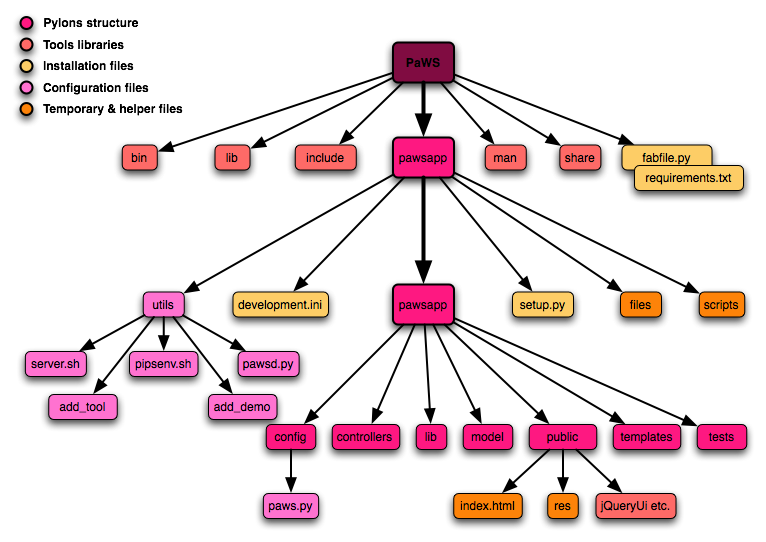
\includegraphics[width=1.0\textwidth]{reportCh2/paws-structure}
  \caption{File structure of PaWS}
  \label{fig:paws_structure}
\end{figure} 

The first one, shown in Figure \ref{fig:paws_structure}, is based on
Pylons directory structure. Files and directories here can
be classified into five types:

\begin{enumerate}

\item {\bf The Pylons} directories which the contain source code
  of PaWS framework. They are described in Section~\ref{architecture_elements}.

\item {\bf The installation files} which are used during the process
  of installation PaWS on a PIPS developper machine. Two of them
  \emph{development.ini} and \emph{setup.py} refer to Pylons directly
  and can be also used as a configuration files. \emph{Fabfile.py} and
  \emph{requirements.txt} are the files of Fabric~\cite{} framework (see
  Section \ref{other_technologies}) designed for quick installation of
  the all dependencies of PaWS framework. More details can be found in
  the section about PaWS installation \ref{installation}.

  \item {\bf The configuration files} - all of the files which can be
    modified by a PIPS developper to get the proper settings for his PaWS
    instance. Scripts used to configurate the application
    content belong to this group too:
    \begin{itemize}
    \item {\bf add\_tool}: a script used to add a new analysis or
      transformation, described in the
      Section~\ref{add_analysis_transformation}.
    \item {\bf add\_demo}: a script used to add a new demonstration,
      described in  Section~\ref{add_demonstration}.
    \item {\bf pipsenv.sh}: a script which adds
      necessary directories to the command path and defines system
      environment variables.
    \item {\bf pawsd.py}: a script which deletes
      old temporary files.
    \item {\bf server.sh}: a script to start application server.
    \end{itemize}

  \item {\bf Temporary and helper files} created by PaWS - directories
    and files which are necessary for PaWS work, but are not the part
    of Pylons architecure. They should not be changed by a PIPS
    developper. Directories \emph{files} and \emph{res} contain
    temporary files created during the PIPS operations. Directory
    \emph{scripts} contains scripts related to adding new
    functionalities of PaWS and the file \emph{index.html} is
    responsible for redirectoring the user to the PaWS introduction
    WEB page.

  \item {\bf Libraries} - directories and files of the tools which
    support work of PaWS, like VirtualEnv, described in
    Section~\ref{virtualenv} or WEB applications technology
    libraries described in Section~\ref{web_application_technologies}.

\end{enumerate}

At the highest level, there are mmostly libraries and binaries related
to the tools used by PaWS, i.e. Virtualenv described in
\ref{virtualenv}.

The second part of PaWS file structure is used for its configuration
by PIPS developper. It is presented in Figure \ref{fig:pips_structure}
and is located in the PIPS \emph{validation} directory. It is mapping
abstract PaWS division into modes, such as tutorial or full control
(described in section \ref{paws_project}) onto the physical
directories structure.

\begin{figure}[h!]
  \centering
  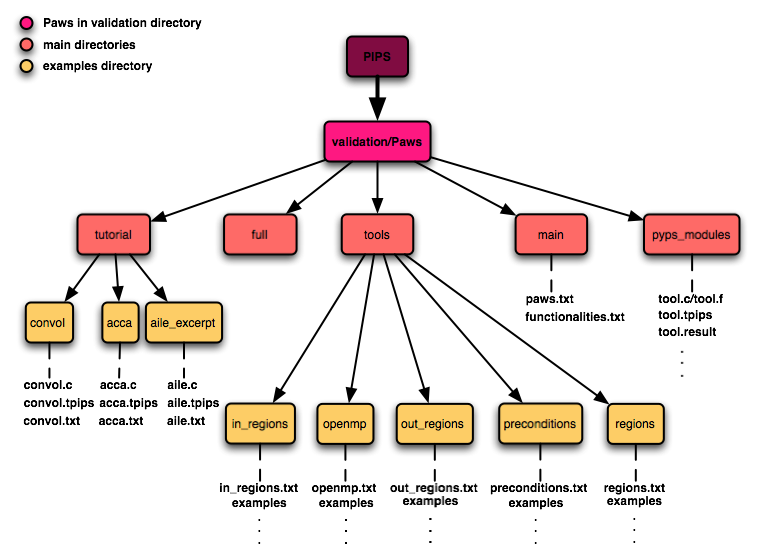
\includegraphics[width=1.0\textwidth]{reportCh2/pips-structure}
  \caption{Structure of PIPS part of PaWS}
  \label{fig:pips_structure}
\end{figure}

\subsection{Architecture elements}
\label{architecture_elements}

This section contains the descriptions of the main types of PaWS
framework elements: controllers, templates, validation directory and
libraries.

\subsubsection{Controllers}

As explained in the previous section, controllers are responsible for
performing actions at the user request. In PaWS several types of
controllers are used.

\begin{enumerate}

\item Controllers responsible for hosting web sites and contains only
  one method ``index''. They are created automatically when adding new
  functionality. Their names correspond to the functionality they
  implement (i.e. ``tools preconditions'' or ``tutorial convol'')

\item Controllers responsible for creating special WEB pages, like the
  ``paas'' controller for the introduction page, or the
  ``descriptions'' controller for extracting information from
  description files.

\item Controllers responsible for the linkage with PyPS or Tpips and
  for performing operations. There are three controllers of this type:
  ``operations'' for basic tools, both at the basic and advanced
  level, ``demo'' for tutorial and ``graph'' for creating dependence
  graps.

\item Controllers for other operations that are not related to PIPS. To
  this group belong the controller ``detector'', which detects the
  language used in source code, and the ``examples'' controller which loads
  supplied examples.

\end{enumerate}

\subsubsection{Templates}

Templates are the files which provide code for WEB pages. They are a
very convenient solution because they let the programmer combine HTML,
Javascript and Python code. What is more, especially when WEB
application consists of many similar pages, templates technology
allows to use the inheritance between templates. That significantly
reduces the amount of redundant code.

PaWS consist of several types of templates:

\begin{itemize}

\item the ``Skeleton'' templates, which provide necessary (and common for
  all of the pages) operations for application to work (like uploading
  files, changing font size or checking if the input source code is
  correct). Those templates (like ``frame'' template) are creating
  structures which are inherited by other, more specific, templates.

\item Templates which are creating frame code dedicated to the
  specific PaWS mode (like tutorial, basic PIPS tools or advanced PIPS
  tools). They are inheriting from more general skeleton templates.

\item Templates which are responsible for creating specific web pages
  dedicated to the special case (one tutorial or PIPS tool). Each of
  them inherits from the appropriate mode template and provides
  characteristic information, such as the name of the PIPS tool or the
  name of a tutorial file.

\item The ``Paas'' template which is responsible for the introduction page,
  and for extracting information about available tools from the
  description files.

\end{itemize}

\subsubsection{Other Modules}
\label{other_modules}

PaWS consists also of some other modules:

\begin{itemize}

\item {\bf \emph{validation}} is the directory of the PIPS project where
  all the supplied examples are placed. All of them
  undergo each day a validation. PaWS validation directory is placed in PIPS
  repository in \emph{validation/Paws} and consists of several
  sub-directories:

  \begin{itemize}

    \item {\bf \emph{pyps\_modules}} described below;

    \item {\bf \emph{tutorial}} which contains all of the demonstration examples;
    \item {\bf \emph{tools}} which contains subdirectories with
      examples dedicated to concrete tool (like \emph{preconditions}
      or \emph{openmp}). Those directories are named after the mode they
      refer to;

  \end{itemize}

\item {\bf PyPS modules} are the part of \emph{validation} directory
  (named \emph{pyps\_modules}). Each module contains PyPS code
  necessary to perform some analysis or transformation. As all of the
  cases kept in \emph{validation} directory because those modules also
  should undergo validation each day.

  \item {\bf \emph{public}} is the Pylons directory where all of the
    helpers but not directly connected to the Pylons or PIPS tools and
    features are placed. In example, all of the Javascript libraries,
    images used by PaWS or description files are stored here.

  \item {\bf \emph{lib}} is the Pylons directory for all of the helper
    Python libraries and modules used by PaWS (like the base Pylons
    controller, the helper for managing files or detection of programming
    languages).

  \item {\bf \emph{tests}} is the Pylons directory for functional
    tests of controllers.

\end{itemize}

\subsection{Flows and scenarios}

This section shows how different elements of PaWS architecture are
linked together. The basic flows for each mode are presented and
described here. Each mode has several cases, different tools or
different demo examples, but in each case the scenario of operations
performed remains the same.

\begin{figure}[h!]
  \centering
  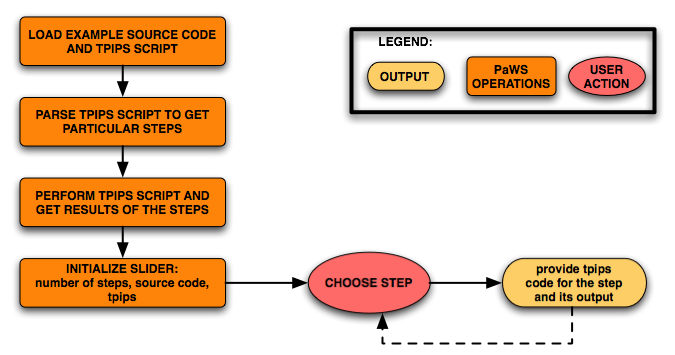
\includegraphics[width=0.7\textwidth]{reportCh2/tutorial_flow}
  \caption{Tutorial flow mode}
  \label{fig:tutorial_flow}
\end{figure}

\begin{itemize}

\item {\bf Demo mode}: there are three scenarios available:
  \emph{aile\_excerpt}, \emph{convol} and \emph{acca-2011}. Input and
  all of the possible operations and their sequence are provided by
  the application - user only controls the step. The basic flow is
  presented on the Picture \ref{fig:tutorial_flow}.
  
  \begin{figure}[h!]
  \centering
  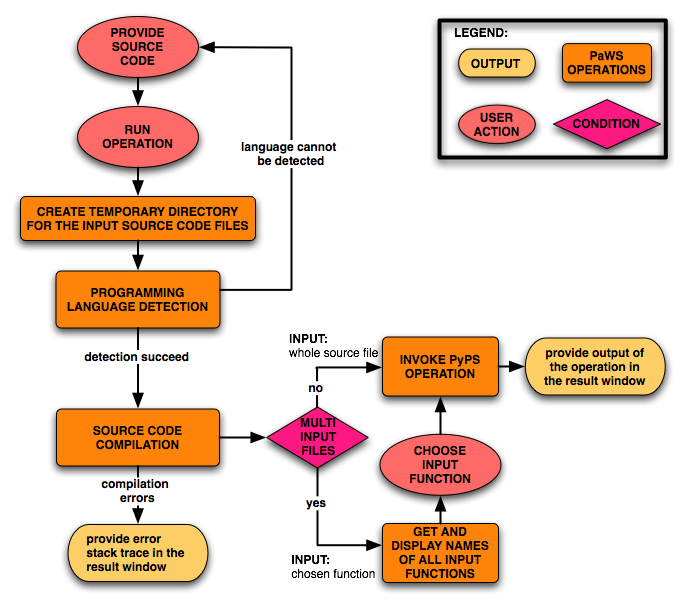
\includegraphics[width=0.7\textwidth]{reportCh2/basic_tool_flow}
  \caption{Basic tool flow mode}
  \label{fig:basic_tool_flow}
\end{figure}

\begin{figure}[h!]
  \centering
  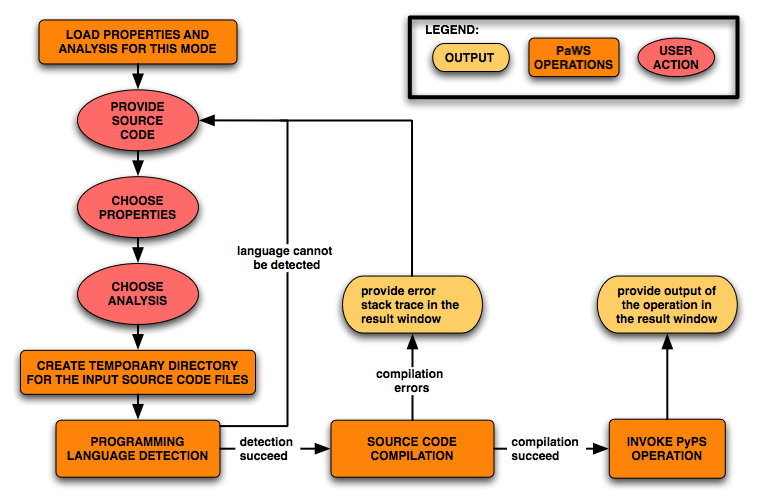
\includegraphics[width=0.7\textwidth]{reportCh2/advanced_tool_flow}
  \caption{Advanced tool flow}
  \label{fig:advanced_tool_flow}
\end{figure}
  
\item {\bf Basic tools - basic level}: five tools are currently
  configured: \emph{preconditions}, \emph{IN regions}, \emph{OUT
    regions}, \emph{regions} and \emph{OpenMP}. This PaWS mode allows
  user to either choose one of supplied examples, different for each
  type of tools, or to provide input source code by him/herself (by
  uploading file or by directly typing or cut-and-pasting in
  application window). The basic flow of this mode is shown in the
  Picture~\ref{fig:basic_tool_flow}.

\item {\bf Basic tools - advanced level}: there are two tools
  available: \emph{preconditions} and \emph{regions}. This mode is
  similar to the basic level - source code can be provided in the same
  way here. The basic scenario is displayed in Picture~\ref{fig:advanced_tool_flow}.
  
  \item {\bf Full control}: not specified and not implemented yet.

\end{itemize}

\section{Selection of the Optimal Architectural Solution}

The selection of the optimal architectural solution and libraries used
to create the framework is not an easy task. Constraints imposed on
the PaWS framework (see Section \ref{design_contraints}) require
design and implementation of a WEB application. It can be done with various
programming languages and libraries.

\subsubsection{Language Selection}

One group of languages used in bigger development projects are Java,
C++ and C\#. Using them requires program compilation and creation of
binary files. Also the programming process requires more programming
work and it is not efficient. What is more, C\# is dedicated to the
Microsoft Windows operation system which disqualifies its use (see
Design Contraints Section \ref{design_contraints}).

The second group of possible languages are scripting languages like
Perl, Python, Ruby and PHP. Perl is an obsolete language, but all of
them are popular as a languages for WEB application design. They are
constantly developed, stay upward-compatible, have a lively community
of developpers, rich documentation, libraries and support. That
explains their popularity.

\subsubsection{WEB Support}

There are three aproaches to create a WEB application using scripting
languages. The first of them is based on CGI\cite{cgi} - Common
Gateway Interface. This technology enables communication between the WEB
server software and and other programs located on the server. The main
disadvantage of this approach is that CGI usually requires the
creation a new process for each request. This is not scalable, it is
not possible to use the same context and global variables for several
requests, and it can cause server load over very quickly. What is more,
CGI does not provide session mechanisms and the Ajax library is not
built-in.

The second possibility is to use template engines like Cheetah
\cite{cheetah} or Jinja2 \cite{jinja2}. The problem is that this
solution is too lightweight - it supports only code generation and not
provides other useful mechanisms such as routing, session variable
handling etc.

The third approach is the most popular approach. It is based on the
Model-View-Controller design pattern (described in Section
\ref{mvc}). This paradigm supports reusability, separation of layers
of the application, is lightweight but easy to extend and takes care
of persistent storage if it is needed. There are a lot of framework
using the MVC pattern like Pylons \cite{pylons}, Django \cite{django}
and Turbogears \cite{turbogears} in Python, Ruby on Rails
\cite{rubyonrails} in Ruby and Symfony \cite{symfony}, CakePHP
\cite{cakephp} and Yii \cite{yii} in PHP.

\subsubsection{WEB Frameworks}

PHP frameworks are more heavyweight and harder to learn than Python
and Ruby ones. The most popular PHP web framework - Symphony also has
problems with compatibility between its versions which makes difficult
to use its support.

Ruby on Rails is a very good framework, but has less support than
Python frameworks, because Ruby is a younger language than
Python. Also Ruby frameworks have performance problems.

The use of Python tools has also other advantages. The main one is the
availability of a Python binding in PIPS framework - PyPS, which can
be use to dynamically perform PIPS operations instead of creating
Tpips (see Section \ref{tpips_interface}) scripts on-the-fly. The
selection of Python enables using PyPS in an easy way, by importing it as
a Python module, but also does not exclude usage of Tpips.

Three Python WEB frameworks were taken into consideration: Pylons,
Django and Turbogears. The last one was rejected because of stability
problems\footnote{TurboGears is based on CherryPy \cite{cherrypy}
  unstable server.}. Despite the fact that Django is more popular than
Pylons, the second one was chosen due to greater flexibility. Pylons
can be extended with any component the user needs, while Django has a
set of its own preferred components. A good example of this problem is
the usage of ORM (Object-relational mapping\cite{orm}). Django does
not allow to use all the available toolkits, like the most popular
one - SQLAlchemy\cite{sqlalchemy}.

Choosing the Pylons tool and its approach to architecture and
structure of the application paid off very quickly - after less than
seven days of work, the first prototype of the application was ready
and able to communicate with PIPS.
%% Very significant fact is that PaWS is not the first CRI project based on Pylons and I could count on strong support from more experienced developers.


\section{Technologies Used}

This section presents an overview of the key technologies used and
their place in the PaWS framework: Tpips, Python, Pylons, Virtual
Environment and Web application technologies (Javascript, Ajax and
JQuery).

\subsection{Tpips}
\label{tpips_interface}

\emph{Tpips} is the line interface and scripting language of the PIPS
project. It allows to use all of PIPS functions in an easy and
user-friendly way, because it simplifies usage of database when
performing operations, it handles all accesses to database, for
instance itself.  Due to using PIPS metavariables, such as \%ALL,
Tpips enables the application of PIPS commands to several modules with
one command. Another advantage of this interface is that it provides
on-line help and automatic completion. Tpips is a great tool for all
tasks which are repeatable and do not require any interaction with the
user.

In the PAWS project, the Tpips interface is used to implement the demo
mode. 
A fixed Tpips script, with a fixed set of PIPS passes, is applied to a
given source file, potentially modified by the user.
%On
%source file, even if it was modified by user, there is Tpips script
%performed with prepared, always the same set of well-known
%operations. 
That allows PaWS to separate the indivudual steps and their
results. They are shown to the user one by one. Also a Tpips script may be
more understandable for new user than Python PyPS code.

\subsection{Python}
\label{python_description}

Python is a portable\footnote{It runs on Windows, Linux/Unix, Mac OS
  and has been ported to the Java and .NET virtual machines} script
programming language. Python is one of the most commonly used
procedural programming languages because of the clearness of its syntax,
its intuitive object orientation, its extensibility provided by modularity -
modules can be written not only in Python but even in C or Java - and its
very high level dynamic data types. One of the major advantages of
Python language is its ability of being used by applications as a
scripting interface.  There is also a lot of tools based on this
language. They are easy to integrate and to extend. It was the main
advantage of using the Pylons Project\cite{pylons} - WEB application
framework technology based on Python. Due to that, PyPS, PIPS Python
interface, could be easily linked to WEB technologies.

\begin{figure}[h!]
  \centering
  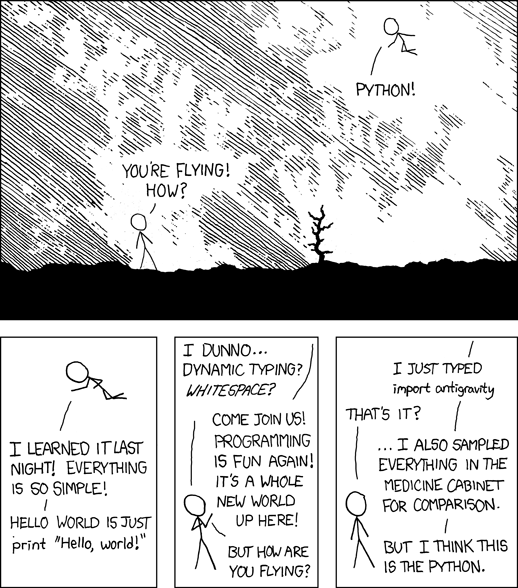
\includegraphics[width=0.6\textwidth]{reportCh2/python}
  \caption{Python by xkcd\cite{python_xkcd}}
  \label{fig:python}
\end{figure}

\subsection{Virtual Environment}
\label{virtualenv}

Virtualenv\cite{virtualenvlit} is the tool used to create isolated
Python environments. Thanks to that, it is possible to make several
distinct environments, which share the same version of Python, but can
have different sets of modules, libraries and packages. All of them
are installed in the Python \emph{site-packages} directory.

This tool is protecting applications against conflicts caused by
different requirements.

\subsection{Pylons}
\label{pylons_descriptions}

Pylons \cite{pylons} is a flexible Python framework based on the
MVC\footnote{MVC stands for \emph{Model-View-Controller}, more in
  section \ref{mvc}} design pattern and WSGI\footnote{WSGI\cite{wsgi}
  stands for \emph{Web Server Gateway Interface} and it is the Python
  standard which specifies interface between web servers and web
  applications.} pattern. Besides its basic WEB application server
functions, Pylons provides also a set of tools and libraries which
extend its way of working, but it does not impose the specific
solutions nor the tools that should be used. The developped can decide
which modules he/she wants to include in his/her application. This
approach guarantees that the application consists only of the
necessary modules and is as light as possible. If it is necessary,
adding third-party libraries is also very easy and intuitive. This
possibility of choosing, adding and composing modules makes Pylons
a very flexible and light framework. It is also very easy to learn and
to use by new developpers.

As written above, Pylons provides a lot of tools which simplify the
development of a WEB application. One of main ones, the
Routes\cite{routes} framework, generates and maps URL addresses to
code. Another tool, WebHelpers\cite{webhelpers} is a set of utility
functions for generating JavaScript\cite{javascript} code. To create
HTML code combined with Python and to pass variables to them, Pylons
is using a \emph{templating system}. It allows user to write HTML and
embed Python code when it is needed\cite{templating_system}. This
solution also supports reusability of the code. The default templating
language is Mako\cite{mako}.

Pylons also can operate on databases, using \emph{Object Relational
  Managers} such as SQLAlchemy\cite{sqlalchemy} or
SQLObject\cite{sqlobject}). In addition it provides caching mechanisms
and manages session variables.

\subsection{Web Application Technologies}
\label{web_application_technologies}

Interactions between users and server are handled by Ajax\cite{ajax}
(Asynchronous JavaScript and XML). Thanks to that technology, the user
view can be refreshed without reloading the whole document. It is
performed in an asynchronous way, which enables user to execute other
operations at the same time. Ajax technology is built in Pylons.


Ajax is used also by JQuery\cite{jquery}, a light and fast library
that contains tools to use Javascript in more advanced ways like
animations or dynamic modifications of site content. Changes provided
by JQuery do not require modifications of the HTML code of the site,
which is important for the developper.

\subsection{Other Tools}
\label{other_technologies}

\begin{itemize}

\item {\bf Pygments}\cite{pygments} is a Python syntax highlighting
  library. It supports a significant number of languages and markup
  formats. There is also a mechanism which allows the developper to
  define his/her own parser to recognize user specific
  languages. Pygments can be used as a library or as a command-line
  tool.

\item {\bf Pyrops} is a Python module based on {\bf pyro}, PYthon
  Remote Objects\cite{pyro}. Pyrops was created as a solution for the
  problem of concurrent accesses to Pips workspaces - it was not
  possible to work on several workspaces at the same time in a
  script\cite{pyps_doc}. Pyrops encapsulate each workspace in a new,
  separate program in a transparent way\footnote{Transparency is
    provided by RPC (and by pyro)\cite{pyps_pass_manager}}. Usage of
  Pyrops is easy for Pyps user - Pyrops workspace inherites of Pyps
  workspace and they are used in the same way.

\item {\bf GCC}\cite{gcc} - the GNU Compiler Collection is one of
  the most popular compiler for C and C++ languages. In PaWS, GCC is
  used for checking the correctness of the user input before performing
  PIPS operations.

\item {\bf F77}\cite{fortran77} and {\bf gFortran}\cite{gfortran} are
  Fortran compilers. They are used in PaWS for the same reason as GCC
  - to check input source code before PIPS is involved.

\item {\bf Fabric}\cite{fabric} - a Python library for automatic
  deployment and setting up of the application. It can be used as a
  library but also as command-line tool. The application developper
  must provide a requirement file where all the dependencies of the
  application and its versions are described. A second file must be
  supplied. It is called \emph{fabfile.py}. It specifies all the
  operations (like setup, installation, clean etc.) that can be used.

%%  \item {\bf versioning}
%%   ??

\end{itemize}




\section{Components Used}
\label{components_used}

This section provides information about specific solutions and
workarounds used in PaWS application.

\begin{itemize}

  \item {\bf Creating graphics} 
  
    Functional requirement No. \ref{req:dependence_graphs} specifies
    that PaWS must be able to create and present dependence graphs. To
    create them in \emph{dot} \cite{dot_format} format\footnote{The
      DOT language is a description language for describing graphs in
      a human and machine readable format.} a PIPS mechanism is used
    (shown in the listing \ref{DotDependenceGraphPrinting}).
  
  \lstset{language=Python,caption={Dependence graph in dot format printing},label=DotDependenceGraphPrinting}
  \begin{lstlisting}
function.print_dot_dependence_graph()
  \end{lstlisting}
  
  A file in \emph{dot} format is transformed into an image in
  \emph{png} format by command \emph{dot} of GraphViz
  Software\cite{graphviz}. Details can be found in \emph{dot} user
  manual: \url{http://www.graphviz.org/pdf/dot.1.pdf}.
  
  \item {\bf Presenting graphics} 
  
    To present dependence graphs, the jQZoom Evolution\cite{jqzoom}
    library is used. This is a light plugin based on JQuery, described
    in \ref{web_application_technologies}. It allows to present the
    image in more user-friendly way. There is small
    thumbnail\footnote{Thumbnail is the small illustration which
      represents the original image at a much smaller size.} shown and
    hoovering mouse over it enables zooming preview of selected part
    of the original, the large image. Moreover this plugin is very easy
    to use, due to its usage of JQuery, and to integrate with PaWS.
  
    The only potential problem of jQZoom usage is the need to provide
    two copies of the image in two sizes: big and thumbnail. To
    fulfill this requirement the Python Image Library (PIL) \cite{pil}
    is used. This is a Python module, which provides all the operations
    dedicated to images processing and supports many files formats. It
    is written in Python and hence is very easy to integrate in the PaWS
    framework. This is its main advantage.
  
  \item {\bf Uploading files}
  
    According to the functional requirement
    No. \ref{req:uploading_files}, PaWS enables user to browse and
    pick his/her own files. Uploading user files caused two problems:

  \begin{itemize}

  \item HTML ``input'' with \emph{type=``file''} used for uploading
    files is not customizable. That means that it is impossible to
    change the style of the button and file name label, which is
    causing aesthetic conflict with the rest of the HTML site.

  \item Uploading files through AJAX requests is impossible because of
    the browsers restrictions and the XmlHttpRequest object
    limitations\cite{ajax_files_upload}. At the same time, PaWS needs
    to be able to upload user files without refreshing the site. Since the
    stardard HTML solution is causing site refreshing, this requires
    the usage of AJAX.

  \end{itemize}
  
  The first problem is easy to solve by creating transparent files
  upload panel which covers false, styled panel (button and file name
  label). Due to that solution, only well styled button and label are
  visible but they are not active - invisible layer of not properly
  styled files upload panel captures users activity.
  
  The second problem is more serious, but it has also been solved. There
  is a hidden, also transparent and invisible, IFrame used as a target
  for file uploading (``target'' attribute is used). When a form with
  the file upload is submitted, the result will be present in a hidden,
  refreshed IFrame, but it can not be seen by user. Content of this
  frame is copied to its proper destination, the visible window. The last
  step is very easy and can be done without refreshing the whole page.
  
  \item {\bf Loading multiple files}
  
    The same requirement No. \ref{req:uploading_files} results in the
    possibility to load several user files packed in one archive file,
    using ``zip'' extension. The only restriction is that all files
    must be written in the same programming language. It is due to
    PyPS framework current limitations.
  
    Python module \emph{zipfile}\cite{zipfile} is used to handle this
    case. It provides archive creating, reading, writing and listing.
  
    For each file, a new tab is created and, when performing an
    operation, the user has to choose one specific function to
    analyse/transform. Dependence graphs are created for all functions
    from all the files.
  
  \item {\bf Printing Result Files}
  
    Functional requirement No.~\ref{req:printing_results} requests the
    possibility of printing the results of the PIPS analyses and
    transformations. To print only the results, not a whole WEB page,
    a special hidden, user invisible frame is used. At user request,
    computation result is loaded into the invisible frame which is
    printed.
  
    There is another possible solution for printing only part of a WEB
    page - usage of special style class which defines which parts of
    the site should be visible when the page is printed. The disadvantage
    of this approach is that it prints all of the page, even if a large
    part of it is invisible, which causes a large wasting of the
    space.
  
  \item {\bf Language detection}
  
    Functional requirement No. \ref{req:language_detection} refers to
    the language detection. It is based on simple tokens
    recognition. It can distinguish between C and Fortran only.
  %% In addition, distinction between different versions of Fortran language (77 and 95) needs compilation.

  %% TO ADD: mechanism! Event when typing source code, pre-compilation
  
  \item {\bf Deleting temporary files}
  
    Most temporary files created during PaWS operations are deleted
    immediately after use. Unfortunately, there are also files which
    need to be kept on the server for a longer time. This applies to
    the files which are used to present results to user, graphs images
    or files with result of transformations and analysis for
    download. To preserve disk space on the server side, requirement
    No. \ref{req:deleting_files}, a cron\footnote{It is a customizable
      Linux job scheduler, which runs periodically user scripts or
      commands\cite{cron}.} task is used. Every hour, a Python script,
    \emph{pawsd.py}, located in \emph{pawsapp$\backslash$utils}
    directory, is invoked to delete all temporary files older than 2
    hours.
  
\end{itemize}

\section{Encountered Problems}
\label{encountered_problems}

PaWS implementation process encountered several problems and bugs:

\begin{itemize}

\item {\bf Perserving the consistency between output of Tpips and Pyps
    computations}
  
  At the beginning operations over prepared examples were performed
  with Tpips script, while user provided code was handled by
  Pyps. Also supplied example after user modification were analyze or
  transformed with Pyps. That was causing a lack of consistency in the
  output - Pyps in the basic level is working with the default values,
  while in the Tpips script other settings can be used as well. Also
  the style of the output pproduced by the Tpips and Pyps is slightly
  different. To provide completely consistent output all operation in
  the tools mode, for basic and for advanced levels, are performed by
  Pyps. Tpips is used in the demonstration mode, which needs script with a
  set of well-defined operations, wnot modifiable by a user.
  
  \item {\bf Validation of the Pyps code}
  
    PIPS and Pyps are constantly in the development process. That can
    cause that the Pyps code used for the PaWS operations might
    require changes according to the Pyps changes. To minimize
    problems resulting from this, such as getting a wrong output or
    being unable to perform operations, all of the Pyps code used in
    PaWS is moved to the \emph{validation} directory, where it can
    undergo validation process and be easily changed if it is needed.
  
  \item {\bf Updating PIPS automatically}
  
    This problem is related to the previous one - PIPS framework,
    which is still changing, has to be updated frequently, to let the
    users try the newest version of it. With automatic update, there
    might be a problem when the current version of PIPS contains bugs or
    is even broken. To avoid such situation, PIPS updates are controlled
    manually.
  
  \item {\bf Provide concurrent access}
  
    The Pylons framework creates a new thread for each user request. This
    might cause problems with Pyps, which requires a new process. Pyrops
    (see Section \ref{other_technologies}) module, which separates
    Pyps workspaces, was the solution of this problem. Pyrops is also
    under development (it is build in Pyps).
  %% bug with sharing workspaces?
  
  \item {\bf Overloading server}
  
    Too many user requests might overload the server. Problem has not
    been solved for the time being.
  
  \item {\bf Points to the documentation}
  
    User should have information about the PIPS properties and
    analyses which might be used in the advanced level of the tools
    mode. The best option to provide it is to link them to the proper
    sections in the PIPS online documentation
    (\url{http://cri.ensmp.fr/pips/pipsmake-rc.htdoc/}). The problem
    is to extract the exact addresses of the sections, whereas they
    are generated randomly and changed during the documentation
    compilation. Currently information about the PIPS settings
    (properties, analyses and phases) is provided by the PaWS
    description files.

\end{itemize}


\section{Conclusion}

Up to now, the architecture and the tools selected have met all the
requirements (see Section \ref{design_requirements}) and design
contraints (see Section \ref{design_contraints}).


